\documentclass{article}

\usepackage{amsmath, amssymb}
\usepackage{graphicx}



\graphicspath{{../figures/}}

\begin{document}

% \tableofcontents

\section{Introduction}

\begin{center}
    {\Huge this is a {\LaTeX}  document}
\end{center}

hello

% % latex table generated in R 4.0.3 by xtable 1.8-4 package
% Wed Apr 21 23:19:25 2021
\begin{table}[ht]
\centering
\begingroup\normalsize
\begin{tabular}{lrrrrrrr}
 \textbf{Variable} & \textbf{Min} & $\mathbf{q_1}$ & $\mathbf{\widetilde{x}}$ & $\mathbf{q_3}$ & \textbf{Max} & $\mathbf{\bar{x}}$ & $\mathbf{s}$ \\ 
  \hline
Annualized GDP Growth Rate (\%) & -31.4 &  1.4 &   3.0 &   4.7 &  33.4 &   3.0 &  4.5 \\ 
  Annualized Inflation (\%) & -19.3 &  1.5 &   3.2 &   5.4 &  24.0 &   3.7 &  3.9 \\ 
  10-year T-bill yield (\%) &   0.6 &  3.9 &   5.7 &   7.7 &  15.3 &   6.0 &  2.9 \\ 
  Shiller P/E Ratio &   6.6 & 15.0 &  20.5 &  25.7 &  44.2 &  20.6 &  8.0 \\ 
  Consumer Confidence Index &  95.7 & 98.9 & 100.5 & 101.1 & 103.1 & 100.0 &  1.6 \\ 
  Market Capitalization-to-GDP Ratio &   0.0 &  0.1 &   0.1 &   0.1 &   0.2 &   0.1 &  0.0 \\ 
  1-Month S\&P 500 Return (\%) & -20.4 & -1.2 &   1.0 &   2.8 &  12.0 &   0.6 &  3.6 \\ 
  3-Month S\&P 500 Return (\%) & -31.1 & -1.7 &   2.4 &   6.2 &  25.9 &   2.0 &  7.0 \\ 
  6-Month S\&P 500 Return (\%) & -37.8 & -2.4 &   4.5 &   9.9 &  38.0 &   4.0 & 10.6 \\ 
  12-Month S\&P 500 Return (\%) & -42.5 & -0.8 &   9.7 &  18.3 &  52.7 &   8.0 & 15.3 \\ 
  60-Month S\&P 500 Return (\%) & -32.6 &  9.4 &  45.4 &  70.4 & 213.9 &  46.1 & 46.5 \\ 
  \end{tabular}
\endgroup
\caption{Summary of features} 
\label{tab:features}
\end{table}


% % latex table generated in R 4.0.3 by xtable 1.8-4 package
% Sun Apr 18 16:32:43 2021
\begingroup\footnotesize
\begin{longtable}{ll|rrr}
 \textbf{Variable} & \textbf{Levels} & $\mathbf{n}$ & $\mathbf{\%}$ & $\mathbf{\sum \%}$ \\ 
  \hline
bubble & 0 & 683 & 93.3 & 93.3 \\ 
   & 1 & 49 & 6.7 & 100.0 \\ 
   \hline
 & all & 732 & 100.0 &  \\ 
   \hline
\hline
\hline
\caption{Bubble distribution} 
\label{tab:imbalance}
\end{longtable}
\endgroup


% latex table generated in R 4.0.3 by xtable 1.8-4 package
% Mon Apr 19 02:01:40 2021
% latex table generated in R 4.0.3 by xtable 1.8-4 package
% Mon Apr 19 02:03:44 2021
\begin{table}[ht]
    \centering
    \begingroup\footnotesize
    \begin{tabular}{lrrrrrr}
     \textbf{Variable} & \textbf{Min} & $\mathbf{q_1}$ & $\mathbf{\widetilde{x}}$ & $\mathbf{q_3}$ & \textbf{Max} & $\mathbf{\bar{x}}$ \\ 
      \hline
    real\_gdp\_growth & -31.4 &  1.4 &   3.0 &   4.7 &  33.4 &   3.0 \\ 
      inflation & -19.3 &  1.5 &   3.2 &   5.4 &  24.0 &   3.7 \\ 
      tbill\_yield &   0.6 &  3.9 &   5.7 &   7.7 &  15.3 &   6.0 \\ 
      shiller\_pe &   6.6 & 15.0 &  20.5 &  25.7 &  44.2 &  20.6 \\ 
      consumer\_confidence &  95.7 & 98.9 & 100.5 & 101.1 & 103.1 & 100.0 \\ 
      mktcap\_gdp\_ratio &   0.0 &  0.1 &   0.1 &   0.1 &   0.2 &   0.1 \\ 
      sp500\_return & -20.4 & -1.2 &   1.0 &   2.8 &  12.0 &   0.6 \\ 
      sp500\_re3 & -31.1 & -1.7 &   2.4 &   6.2 &  25.9 &   2.0 \\ 
      sp500\_re6 & -37.8 & -2.4 &   4.5 &   9.9 &  38.0 &   4.0 \\ 
      sp500\_re12 & -42.5 & -0.8 &   9.7 &  18.3 &  52.7 &   8.0 \\ 
      sp500\_re60 & -32.6 &  9.4 &  45.4 &  70.4 & 213.9 &  46.1 \\ 
      \end{tabular}
    \endgroup
    \caption{Summary of features} 
    \label{tab:features}
    \end{table}


% Table created by stargazer v.5.2.2 by Marek Hlavac, Harvard University. E-mail: hlavac at fas.harvard.edu
% Date and time: Sun, Apr 18, 2021 - 16:40:33
\begin{table}[!htbp] \centering 
  \caption{} 
  \label{tab:logit} 
\begin{tabular}{@{\extracolsep{5pt}}lc} 
\\[-1.8ex]\hline 
\hline \\[-1.8ex] 
 & \multicolumn{1}{c}{\textit{Dependent variable:}} \\ 
\cline{2-2} 
\\[-1.8ex] & bubble \\ 
\hline \\[-1.8ex] 
 real\_gdp\_growth & 0.012 \\ 
  & (0.034) \\ 
  & \\ 
 inflation & 0.093$^{***}$ \\ 
  & (0.028) \\ 
  & \\ 
 tbill\_yield & 0.234$^{***}$ \\ 
  & (0.071) \\ 
  & \\ 
 shiller\_pe & $-$0.661$^{***}$ \\ 
  & (0.058) \\ 
  & \\ 
 consumer\_confidence & $-$1.279$^{***}$ \\ 
  & (0.154) \\ 
  & \\ 
 mktcap\_gdp\_ratio & 217.538$^{***}$ \\ 
  & (18.556) \\ 
  & \\ 
 sp500\_return & $-$0.092$^{***}$ \\ 
  & (0.033) \\ 
  & \\ 
 sp500\_re3 & 0.034 \\ 
  & (0.022) \\ 
  & \\ 
 sp500\_re6 & $-$0.049$^{**}$ \\ 
  & (0.019) \\ 
  & \\ 
 sp500\_re12 & $-$0.126$^{***}$ \\ 
  & (0.015) \\ 
  & \\ 
 sp500\_re60 & 0.077$^{***}$ \\ 
  & (0.006) \\ 
  & \\ 
 Constant & 115.874$^{***}$ \\ 
  & (14.361) \\ 
  & \\ 
\hline \\[-1.8ex] 
Observations & 1,103 \\ 
Log Likelihood & $-$411.350 \\ 
Akaike Inf. Crit. & 846.699 \\ 
\hline 
\hline \\[-1.8ex] 
\textit{Note:}  & \multicolumn{1}{r}{$^{*}$p$<$0.1; $^{**}$p$<$0.05; $^{***}$p$<$0.01} \\ 
\end{tabular} 
\end{table} 


% latex table generated in R 4.0.3 by xtable 1.8-4 package
% Sun Apr 18 20:24:34 2021
\begin{table}[ht]
\centering
\begin{tabular}{rllll}
  \hline
 & Model & Sensitivity & Specificity & Balanced Accuracy \\ 
  \hline
1 & Logit-P & 0.727 & 0.721 & 0.724 \\ 
  2 & Logit-RW & 0.727 & 0.735 & 0.731 \\ 
  3 & RF-CV & 1 & 0.86 & 0.93 \\ 
  4 & RF-RW & 0.455 & 1 & 0.727 \\ 
  5 & RNN-BiLSTM-focal & 0 & 1 & 0.5 \\ 
   \hline
\end{tabular}
\caption{The peformance of models} 
\label{tab:res}
\end{table}


% latex table generated in R 4.0.3 by xtable 1.8-4 package
% Sun Apr 18 19:24:41 2021
\begin{table}[ht]
\centering
\begin{tabular}{rrrrr}
  \hline
 & 0.005 & 0.01 & 0.015 & 0.05 \\ 
  \hline
3 & 0.67 & 0.68 & 0.72 & 0.80 \\ 
  5 & 0.91 & 0.99 & 0.86 & 0.85 \\ 
  6 & 0.99 & 0.94 & 0.86 & 0.90 \\ 
  7 & 0.97 & 0.96 & 0.88 & 0.90 \\ 
  12 & 0.97 & 0.93 & 0.91 & 0.88 \\ 
   \hline
\end{tabular}
\caption{Balanced accuracy of RF-CV with different quantiles (column) and periods (row)} 
\label{tab:rob}
\end{table}



% \begin{figure}
%     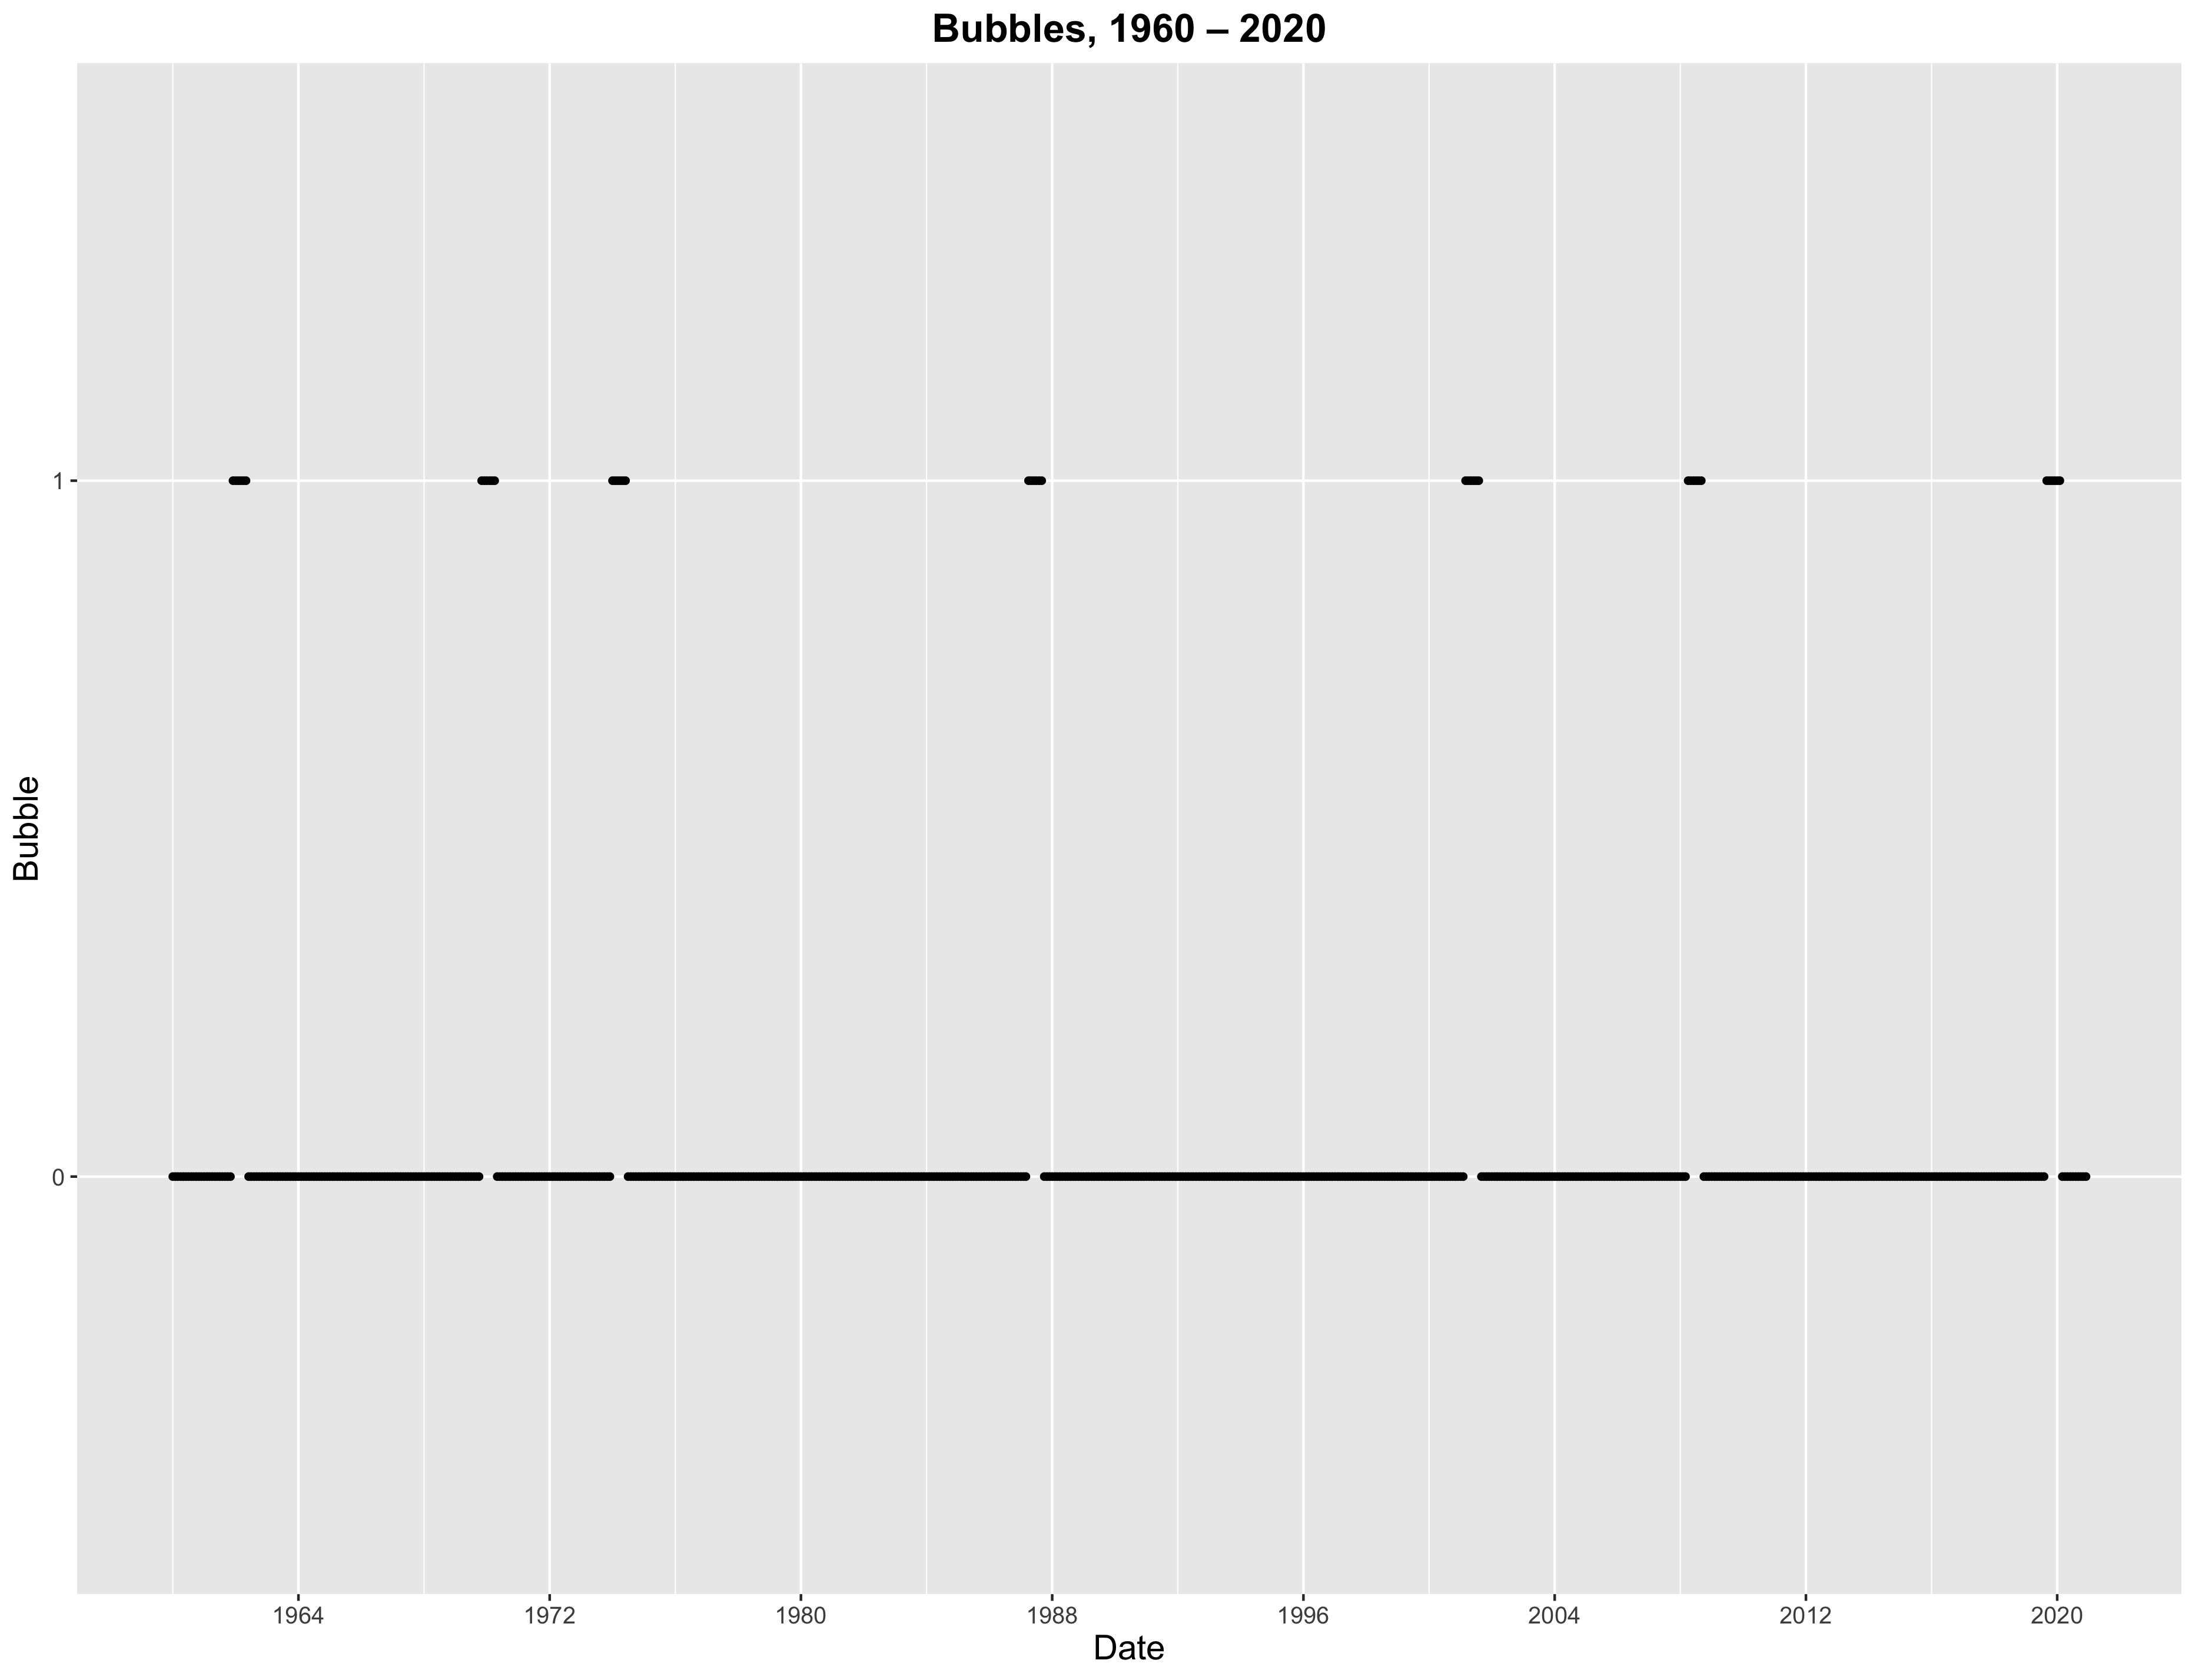
\includegraphics[scale=0.01]{bubble_def.png} 
% \end{figure}

\textbf{hello}
\textit{hello}
\emph{test}
hello world
hello world
what do you think is the future of the world

this is the future of our life
\[f(x) = (x+2) ^3 \]
\(f(x) = x\)

\begin{align}
    f(x) = x \\
    1 + 1_2
    \left( hello \right)
\end{align}

\[
\begin{pmatrix}
    a_{11} & a_{12} \\
    a_{21} & a_{22}
\end{pmatrix}
\]

\begin{tabular}{lll}
    a & b c & d\\ 
    a & d & c
    
\end{tabular}
\end{document}

